\documentclass[table]{beamer}
\usepackage[utf8]{inputenc}
\usepackage[brazilian]{babel}
\usepackage{amsmath}
\usepackage{graphicx}
\usepackage{hyperref}
\usepackage{ragged2e}   
\usepackage{epstopdf}
\usepackage{multirow}
\usepackage{minted}
\usepackage{booktabs}

\setbeamertemplate{sidebar right}{}
\setbeamertemplate{footline}{%
\hfill\usebeamertemplate***{navigation symbols}
\hspace{1cm}\insertframenumber{}/\inserttotalframenumber}

\addtobeamertemplate{block begin}{}{\justifying}  %new code

\setbeamertemplate{footline}
{
  \leavevmode%
  \hbox{%
  \begin{beamercolorbox}[wd=.333333\paperwidth,ht=2.25ex,dp=1ex,center]{author in head/foot}%
    \usebeamerfont{author in head/foot}\insertsection
  \end{beamercolorbox}%
  \begin{beamercolorbox}[wd=.333333\paperwidth,ht=2.25ex,dp=1ex,center]{title in head/foot}%
    \usebeamerfont{title in head/foot}\insertsubsection
  \end{beamercolorbox}%
  \begin{beamercolorbox}[wd=.333333\paperwidth,ht=2.25ex,dp=1ex,right]{date in head/foot}%
    \usebeamerfont{date in head/foot}\insertshortdate{}\hspace*{2em}
    \insertframenumber{} / \inserttotalframenumber\hspace*{2ex} 
  \end{beamercolorbox}}%
  \vskip0pt%
}

\begin{document}

\begin{frame}
   \frametitle{Compiladores}
   \large
   \begin{center}
   Análise Sintática Descendente
   \end{center}
   \scriptsize
   \begin{center}
      João Marcelo Uchôa de Alencar \\
      joao.marcelo@ufc.br \\
      UFC-Quixadá
   \end{center}
\end{frame}

\begin{frame}
   \tableofcontents
\end{frame}

\begin{frame}
   \frametitle{Análise Sintática Descendente}
   \begin{itemize}
      \item Analisa a cadeia de marcas através da \textbf{derivação à esquerda};
      \item a árvore de análise é percorrida em \textbf{pré-ordem};
      \item \textbf{analisador com retrocesso}: testa diferentes possibilidades;
      \item \textbf{analisador preditivo}: baseado na leitura de uma ou mais marcas;
      \begin{itemize}
         \item descendentes recursivos;
	 \item LL(1).
      \end{itemize}
      \item vamos estudar os preditivos.
   \end{itemize}
   \centering
   
\includegraphics[scale=0.15]{figuras/previsao.jpg}
\end{frame}

\section{Análise Sintática Descendente Recursiva}
\begin{frame}
   \frametitle{O Método Descendente Recursivo Básico}
   \begin{block}{Metodologia}
      \begin{enumerate}
         \item A regra gramatical de um não terminal é usada para definir um procedimento;
	 \item sequências de terminais correspondem a casamento da entrada;
	 \item sequências de não terminais correspodem a ativações de outros procedimentos;
	 \item a alternância corresponde a declarações de \textit{if} ou \textit{case}.
      \end{enumerate}
   \end{block}
\end{frame}

\begin{frame}[fragile]
   \frametitle{O Método Descendente Recursivo Básico}
   \begin{columns}
   \begin{column}{0.5\textwidth}
   $\textit{exp} \to \textit{exp soma termo} | \textit{termo}$ \\
   $\textit{soma} \to +|-$ \\
   $\textit{termo} \to \textit{termo mult fator} | \textit{fator}$ \\
   $\textit{mult} \to *$ \\
   $\textit{fator} \to (\textit{exp}) | \textbf{número}$
   \end{column}
   \begin{column}{0.5\textwidth}
   \begin{minted}{pascal}
   procedure fator;
   begin
      case marca of
      ( : casamento(();
          exp;
	  casamento());
      numero:
          casamento(numero);
      else: erro;
      end case;
   end fator;
   \end{minted}
   \end{column}
   \end{columns}
\end{frame}

\begin{frame}[fragile]
   \frametitle{O Método Descendente Recurso Básico}
   \small
   \begin{columns}
   \begin{column}{0.5\textwidth}
   \begin{minted}{pascal}
procedure casamento 
         (marcaEsperada);
begin
   if marca = marcaEsperada then
      capturaMarca;
   else
      erro;
   end if;
end casamento;
   \end{minted}
   \end{column}
   \begin{column}{0.5\textwidth}
   \begin{itemize}
      \item Por enquanto, não definimos \textit{erro};
      \item assumimos \textit{exp} e \textit{termo} definidos;
      \item como esses não terminais não tem terminais na sua definição, não é tão fácil construir seus procedimentos;
      \item vamos usar a EBNF.
   \end{itemize}
   \end{column}
   \end{columns}
\end{frame}

\begin{frame}[fragile]
   \frametitle{Repetição e Escolha: o Uso da EBNF}
   \textit{if-decl} $\to$ \textbf{if} (\textit{exp}) \textit{declaração} \\
   $|$ \textbf{if} (\textit{exp}) \textit{declaração} \textbf{else} \textit{declaração}
   \begin{columns}
   \begin{column}{0.5\textwidth}
   \begin{minted}{pascal}
procedure declIf;
begin
   casamento(if);
   casamento(();
   exp;
   casamento());
   declaracao;
   if marca = else then
      casamento(else);
      declaracao;
   end if;
end declIf;
   \end{minted}
   \end{column}
   \begin{column}{0.5\textwidth}
   \textit{if-decl} $\to$ \textbf{if} (\textit{exp}) \textit{declaracao} [ \textbf{else} \textit{declaracao} ]
   \begin{itemize}
      \item Ambas opções começa com \textbf{if};
      \item por isso, usamos a EBNF;
      \item os colchetes são traduzidos em testes;
      \item a gramática é ambígua, mas o procedimento trata esse problema.
   \end{itemize}
   \end{column}
   \end{columns}
\end{frame}

\begin{frame}[fragile]
   \frametitle{Repetição e Escolha: o Uso da EBNF}
   \begin{center}
   \textit{exp} $\to$ \textit{exp soma termo} $|$ \textit{termo}
   \end{center}
   \begin{itemize}
      \item Usando a metodologia, \textit{exp} invocaria \textit{exp}!
      \item Um teste para escolher entre \textit{exp} e \textit{termo} é problemático;
      \item ambos pode resultar em ( ou \textbf{número}.
   \end{itemize}
   \begin{center}
   \textit{exp} $\to$ \textit{termo} \{ \textit{soma termo} \}
   \end{center}
   \begin{minted}{pascal}
procedure exp;
begin 
   termo;
   while marcar = + or marca = - do
      casamento(marca);
      termo;
   end while;
end exp;
   \end{minted}
\end{frame}

\begin{frame}[fragile]
   \frametitle{Repetição e Escolha: o Uso da EBNF}
   \begin{center}
   \textit{termo} $\to$ \textit{fator} \{ \textit{mult fator} \}
   \end{center}
   \begin{minted}{pascal}
procedure termo;
begin
   fator;
   while marca = * do
      casamento(marca);
      fator;
   end while;   
end termo;
   \end{minted}
\end{frame}

\begin{frame}[fragile]
   \frametitle{Gramática de Aritmética de Inteiros}
   \begin{minted}{pascal}
function exp:inteiro;
var temp:inteiro;
begin
   temp := termo;
   while marca = + or marca = - do
      case marca of
      + : casamento(+);
          temp := temp + termo; 
      - : casamento(-);
          tempo := temp - termo;
      end case;	  
   end while;
end exp;
   \end{minted}
\end{frame}

\begin{frame}[fragile]
   \frametitle{Gramática de Aritmética de Inteiros}
   \begin{minted}{c}
#include <stdio.h>
#include <stdlib.h>

char token; /* variável de marca global */
/* protótipos de funções para ativações recursivas */
int exp(void);
int term(void);
int fator(void);
void error(void) {
   fprintf(stderr, "Erro\n");
   exit(1);
}
void match(char expectedToken) {
   if (token == expectedToken) token = getchar();
   else error();
}
   \end{minted}
\end{frame}

\begin{frame}[fragile]
   \frametitle{Gramática de Aritmética de Inteiros}
   \begin{minted}{c}
 int main(int argc, char *argv[]) {
   int result;
   token = getchar(); /* carrega a marca com o primeiro 
                         caractere para verificação 
			 à frente */

   result = exp();
   if (token == '\n') /* teste final de linha */
      printf("Resultado = %d\n", result);
   else error(); /* caracteres indevidos na linha */
   return 0;
}
   \end{minted}
\end{frame}

\begin{frame}[fragile]
   \frametitle{Gramática de Aritmética de Inteiros}
   \begin{minted}{c}
 int exp(void) {
   int temp = term();
   while ((token == '+') || (token == '-'))
      switch(token) {
         case '+' : match('+');
	            temp += term();
		    break;
         case '-' : match('-');
	            temp -= term();
		    break;
      }
   return temp;
}
   \end{minted}
\end{frame}

\begin{frame}[fragile]
   \frametitle{Gramática de Aritmética de Inteiros}
   \begin{minted}{c}
 int term(void) {
   int temp = factor();
   while (token == '*') {
      match('*');
      temp *= factor();
   }
   return temp;
}
   \end{minted}
\end{frame}

\begin{frame}[fragile]
   \frametitle{Gramática de Aritmética de Inteiros}
   \begin{minted}{c}
  int factor(void) {
   int temp;
   if (token == '(') {
      match('(');
      temp = exp();
      match(')');
   } else if (isdigit(token)) {
      ungetc(token, stdin);
      scanf("%d", &temp);
      token = getchar();
   }
   else error();
   return temp;
} 
   \end{minted}
\end{frame}

\begin{frame}
   \frametitle{E as Árvores?}
   \begin{itemize}
      \item A metodologia adotada mostra como reconhecer uma cadeia da gramática, mas não trata da definição das árvores;
      \item a associatividade foi mantida porque os cálculos foram feitos durante o reconhecimento;
      \item em um compilador, precisamos construir a árvore para garantir a associatividade, já que a execução ocorre em outro momento.
   \end{itemize}
   \centering
   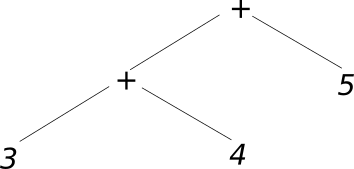
\includegraphics[scale=0.5]{figuras/arvore_abstrata.png} \\
   \vspace{1.0cm}
   Para a expressão $3+4+5$, o nó que representa $3+4$ deve ser criado antes do nó que representa a adição de 5.
\end{frame}

\begin{frame}[fragile]
   \frametitle{Construção de Árvores Sintáticas}
   \small
   \begin{minted}{pascal}
function exp: arvoreSintatica;
var temp, novatemp, arvoreSintatica;
begin
   temp := termo;
   while marca = + or marca = - do
      case marca of
         + : casamento(+);
	     novatemp := criaNoOp(+);
	     filhoEsq(novatemp) := temp;
	     filhoDir(novatemp) := termo;
	     temp := novatemp;
	 - : casamento(-);
	     novatempo := criaNoOp(-);
	     filhoEsq(novatemp) := temp;
	     filhoDir(novatemp) := termo;
	     temp := novatemp;
      end case;
   end while;
end exp;
   \end{minted}
\end{frame}

\begin{frame}[fragile]
   \frametitle{Construção de Árvores Sintáticas - If Then Else}
   \small
   \begin{minted}{pascal}
function declaracaoIf: arvoreSintatica;
var temp : arvoreSintatica;
begin
   casamento(if);
   casamento(();
   temp := criaNoDecl(if);
   testeFilho(temp) := exp;
   casamento());
   thenFilho(temp) := declaracao;
   if marca = else then
      casamento(else);
      elseFilho(temp) := declaracao;
   else
      elseFilho(temp) := nil;
   end if;
end declaracaoIf;
   \end{minted}
\end{frame}

\begin{frame}
   \frametitle{Limitações}
   \begin{itemize}
      \item Nem sempre é fácil converte de BNF para EBNF;
      \item na regra $A\to \alpha | \beta$, se $\alpha$ e $\beta$ iniciarem com os mesmos não terminais, como decidir?
      \item \textbf{conjuntos primeiros} $\alpha$ e $\beta$: conjuntos de marcas que podem iniciar legamente cada cadeia de caracteres;
      \item \textbf{conjunto sequência} de A: quais marcas podem suceder legalmente o não terminal A.
   \end{itemize}
\end{frame}

\section{Análise Sintática LL(1)}
\begin{frame}
   \frametitle{Análise Sintática LL(1)}
   Vamos evitar a recursão com o uso de uma \textbf{pilha}! \\
   \begin{center}
   \textit{S} $\to$ (\textit{S})\textit{S} $|$ $\varepsilon$
   \end{center}
   Processando a cadeia \textit{()}:
   \begin{table}
      \begin{tabular}{c|l|r|c}
      & Pilha & Entrada & Ação \\
      \hline 
      1 & \$\textit{S}    & ()\$           & \textit{S} $\to$ (\textit{S})\textit{S}  \\
      2 & \$\textit{S)S(} & ()\$           & casamento      \\
      3 & \$\textit{S)S}  & )\$            & $S\to \varepsilon$      \\
      4 & \$\textit{S)}   & )\$            & casamento      \\
      5 & \$\textit{S}    & \$             & $S\to \varepsilon$      \\
      6 & \$              & \$             & aceita      \\
      \hline
      \end{tabular}
   \end{table}
   Aceitação garantida se a pilha e a entrada ficarem vazias.
\end{frame}

\begin{frame}
   \frametitle{Análise Sintática LL(1)}
   Um analisador sintático descendente substitui um não terminal no topo da pilha por uma de suas escolhas na regra gramatical (em BNF).
   \begin{block}{Ações:}
      \begin{enumerate}
         \item \textbf{gera}: substituir um não terminal $A$ no topo da pilha por uma cadeia $\alpha$ com base na escolha da regra $A\to\alpha$;
	 \item \textbf{casamento}: casar uma marca no topo da pilha com a marca de entrada seguinte.
      \end{enumerate}
   \end{block}
   \begin{itemize}
      \item As inserções na pilha equivalem aos passos de uma derivação;
      \item no lugar as ações, podemos ter procedimentos que constroem a árvore sintática.
   \end{itemize}
\end{frame}

\begin{frame}
   \frametitle{A Tabela e o Algoritmo LL(1)}
   \begin{itemize}
      \item Com um não terminal $A$ no topo da pilha, precisamos escolher qual regra de $A$ para colocar na pilha com base na marca corrente da entrada;
      \item se marca na pilha for igual a marca da entrada, temos o \textit{casamento}, se forem diferentes, erro;
      \item vamos listar as escolhas em uma tabela chamada $M[N, T]$:
      \begin{itemize}
         \item $N$ são os não terminais;
	 \item $T$ são os terminais mais o símbolo \$.
      \end{itemize}
   \end{itemize}
\end{frame}

\begin{frame}
   \frametitle{A Tabela e o Algoritmo LL(1)}
   \begin{block}{Regras de Construção da Tabela}
      \begin{enumerate}
         \item Se $A\to\alpha$ for uma escolha de produção, e houver derivação $\alpha\Rightarrow^{*}a\beta$, na qual $a$ é uma marca, acrescente $A\to\alpha$ à célula da tabela $M[A, a]$;
	 \item se $A\to\alpha$ for uma escolha de produção, e houver derivações $\alpha\Rightarrow^{*}\varepsilon$ e $S\$\Rightarrow^{*}\beta Aa\gamma$, nas quais $S$ é símbolo de começo e $a$ é uma marca, acrescente $A\to\alpha$ à célula $M[A,a]$.
      \end{enumerate}
   \end{block}
   \begin{block}{Motivação das Regras}
      \begin{enumerate}
         \item Dada uma marca $a$ na entrada, queremos selecionar uma regra $A\to\alpha$, se $\alpha$ puder produzir $a$ para casamento;
	 \item se $A$ derivar a cadeia vazia (via $A\to\alpha$), e se $a$ for uma marca que possa suceder legalmente A em uma derivação, então selecionamos $A\to\alpha$ para se livrarmos do $A$.
      \end{enumerate}
   \end{block}
\end{frame}

\begin{frame}
   \frametitle{A Tabela e o Algoritmo LL(1)}
   \begin{center}
   \textit{S} $\to$ (\textit{S})\textit{S} $|$ $\varepsilon$
   \end{center}
   \begin{itemize}
      \item Pela regra 1, $M[S, (]$ aponta para $S\to(S)S$;
      \item Pela regra 2, considerando $S\Rightarrow(S)S$, $\alpha=\varepsilon$, $\beta=($, $A=S$, $a=)$, e $\gamma=S\$$, podemos incluir $S\to\varepsilon$ em $M[S,)]$;
      \item como $S\$\Rightarrow^{*}S\$$, podemos adicionar $S\to\varepsilon$ à $M[S,\$]$. 
   \end{itemize}

   \begin{table}
      \begin{tabular}{l|c c c}
      M[N,T]& ( & ) & \$\\
      \hline 
      S & $S\to(S)S$ & $S\to\varepsilon$ & $S\to\varepsilon$ \\
      \end{tabular}
   \end{table}
\end{frame}

\begin{frame}[fragile]
   \frametitle{A Tabela e o Algoritmo LL(1)}
   \footnotesize
   Uma gramática é uma \textbf{gramática LL(1)} se a tabela de análise sintática LL(1) associada tiver no máximo uma produção em cada célula.
   \scriptsize
   \begin{minted}{text}
(* assume que $ marca o fim da pilha e da entrada *)
coloca o símbolo de começo no topo da pilha;
while topo da pilha != $ and próxima marca for != $ do 
   if topo da pilha for o terminal a
      and próxima marca de entrada for a
   then (* casamento *)
      retira da pilha;
      avança entrada;
   else if topo da pilha for um não terminal A
        and próxima marca de entrada for terminal a
	and célula da tabela M[A,a] contiver a produção
	    A -> X1X2...Xn
	then (*gera*)
	   retira da pilha;
	   for i := n downto 1 do
	      coloca Xi na pilha;
	else erro;
if topo da pilha for igual a $
   and marca seguinte na entrada for igual a $
then aceita
else erro;
   \end{minted}
\end{frame}

\begin{frame}
   \frametitle{A Tabela e o Algoritmo LL(1)}
   \textit{declaração} $\to$ \textit{if-decl} $|$ \textbf{outra} \\
   \textit{if-decl} $\to$ \textbf{if (} \textit{exp} \textbf{)} \textit{declaração} \textit{else-parte} \\ 
   \textit{else-parte} $\to$ \textbf{else} \textit{declaração} $| \varepsilon$ \\
   \textit{exp} $\to$ \textbf{0} $|$ \textbf{1}
   \begin{block}{Questões}
      \begin{itemize}
         \item Como ficaria a tabela?
	 \item Como seria a execução para \textbf{if} (0) \textbf{if} (1) outra \textbf{else} outra?
      \end{itemize}
   \end{block}
\end{frame}

\begin{frame}
   \frametitle{A Tabela e o Algoritmo LL(1)}
   \tiny
   \begin{table}
      \begin{tabular}{l|l|l|l|l|l|l}
      \hline
      $M[N,T]$ & \textbf{if} & outra & \textbf{else} & 0 & 1 & \$ \\
      \hline 
      \textit{declaração} & \textit{declaração} $\to$ & \textit{declaração} $\to$ & & & & \\  
       & \textit{if-decl} & \textit{outra} & & & & \\  
      \hline
      \textit{if-decl} & \textit{if-decl} $\to$ & & & & & \\  
      & \textbf{if} (\textbf{exp}) & & & & & \\  
      & \textit{declaração} & & & & & \\  
      & \textit{else-parte} & & & & & \\  
      \hline
      \textit{else-parte} & & &\textit{else-parte} $\to$ & & & \textit{else-parte} $\to \varepsilon$ \\  
      & & &\textbf{else} & & & \\  
      & & &\textit{declaração} & & & \\  
      & & &\textit{else-parte} $\to \varepsilon$ & & & \\  
      \hline
      \textit{exp} & & & &\textit{exp} $\to 0$ & \textit{exp} $\to 1$ & \\  
      \end{tabular}
   \end{table}
   \normalsize
   A entrada $M[\textit{else-parte},\textbf{else}]$ contém duas opções. A gramática é ambígua e não é LL (1). \\
   Podemos manualmente alterar o algoritmo para escolher sempre a primeira produção.
\end{frame}

\begin{frame}
   \frametitle{Remoção de Recursão e Fatoração à Esquerda}
   \begin{itemize}
      \item Não podemos resolver os problemas da repetição e escolha na LL(1) transformando a gramática para a notação EBNF;
      \item \textbf{remoção da recursão à esquerda};
      \item \textbf{remoção da fatoração à esquerda};
      \item não há garantias de transformação em LL(1), mas funciona na maioria dos casos para gramáticas de linguagem de programação.
   \end{itemize}
\end{frame}

\begin{frame}
   \frametitle{Remoção de Recursão à Esquerda}
   \begin{block}{Caso 1: recursão imediata à esquerda simples}
   \textit{A} $\to$ \textit{A} $\alpha|\beta$ se transforma em: \\
   \textit{A} $\to \beta$ $\textit{A}^{'}$ \\
   $\textit{A}^{'} \to \alpha \textit{A}^{'} | \varepsilon$ \\
   Lembrando que $\alpha$ e $\beta$ são cadeias de terminas ou não terminais e $\beta$ não começa com \textit{A}.
   \end{block}
   \begin{block}{Exemplo}
   \textit{exp} $\to$ \textit{exp soma termo} $|$ \textit{termo}
   \end{block}
\end{frame}

\begin{frame}
   \frametitle{Remoção de Recursão à Esquerda}
   \begin{block}{Caso 2: recursão imediata à esquerda geral}
   \textit{A} $\to$ $\textit{A}\alpha_{1}|\textit{A}\alpha_{2}|\text{...}|\textit{A}\alpha_{n}|\beta_{1}|\beta_{2}|\text{...}|\beta_{m}$, em que nenhum $\beta$ começa com \textit{A}, se transforma em: \\
   $\textit{A}\to \beta_{1}\textit{A}^{'}|\beta_{2}\textit{A}^{'}|\text{...}|\beta_{m}\textit{A}^{'}$\\
   $\textit{A}^{'} \to \alpha_{1}\textit{A}^{'}|\alpha_{2}\textit{A}^{'}|\text{...}|\alpha_{n}\textit{A}^{'}|\varepsilon$
   \end{block}
   \begin{block}{Exemplo}
   \textit{exp} $\to$ \textit{exp} + \textit{termo} $|$ \textit{exp} - \textit{termo} $|$ \textit{termo}
   \end{block}
\end{frame}

\begin{frame}[fragile]
   \frametitle{Remoção de Recursão à Esquerda}
   \begin{block}{Caso 3: recursão à esquerda geral}
\textbf{for} i:= 1 \textbf{to} m \textbf{do} \\
\hspace{0.4cm} \textbf{for} j:=1 \textbf{to} $i - 1$ \textbf{do} \\
\hspace{1.0cm} substituir cada escolha de regra gramatical da forma $A_{i} \to A_{j}\beta$ pela regra $A_{i} \to \alpha_{1}\beta | \alpha_{2}\beta | \text{...} | \alpha_{k}\beta$, onde $A_{i} \to \alpha_{1} | \alpha_{2} | \alpha_{k}$ é a regra corrente para $A_{j}$; \\
\hspace{0.4cm} \textbf{end for} \\
\hspace{0.4cm} remover a recursão imediata à esquerda de $A_{i}$; \\
\textbf{end for}
   \end{block}
   \begin{block}{Exemplo}
   $A \to Ba | Aa | c$\\
   $B \to Bb | Ab | d $
   \end{block}
\end{frame}

\begin{frame}
   \frametitle{Remoção de Recursão à Esquerda}
   $ exp \to exp^{'}$ \\
   $ exp^{'} \to \textit{soma termo } exp^{'} | \varepsilon $ \\
   $ soma \to +|-$ \\
   $ termo \to \textit{fator } termo^{'}$ \\
   $ termo^{'} \to \textit{mult fator } termo^{'} | \varepsilon $ \\
   $ mult \to * $ \\
   $ fator \to (exp) | \textbf{número} $
   \begin{itemize}
      \item A gramática agora é LL(1), somente BNF;
      \item o problema é que alteramos a associatividade à esquerda da subtração ou adição;
      \item considere árvore de análise de 3 - 4 - 5;
      \item por isso, apesar de úteis, gramáticas LL(1) não resolvem todos os problemas.
   \end{itemize}
\end{frame}

\begin{frame}
   \frametitle{Fatoração à Esquerda}
   $A \to \alpha\beta|\alpha\gamma$ \\
   $\alpha$ é o mesmo prefixo, impossibilitando a escolha da produção. A solução é transformar em: \\
   $A \to \alpha A^{'}$ \\
   $A^{'} \to \beta | \gamma$
   \begin{block}{Exemplos}
      \begin{enumerate}
         \item $\textit{decl-sequência} \to decl; \textit{decl-sequência} | decl$ \\
	 $decl \to s$
	 \item $\textit{if-decl} \to if (exp) \textit{declaração} | if (exp) \textit{declaração else  declaração}$
	 \item $exp \to termo + exp | termo $
	 \item $\textit{declaração} \to \textit{atribuição-decl} | \textit{ativação-decl} | \textbf{outra}$ \\
	 $\textit{atribuição-decl} \to \textbf{identificador} := exp$ \\
	 $\textit{ativação-decl} \to \textbf{identificador} (\textit{exp-list})$ 
      \end{enumerate}
   \end{block}
\end{frame}

\section{Conjuntos Primeiros e de Sequência}
\begin{frame}
   \frametitle{Conjuntos Primeiros e de Sequência}
   \begin{itemize}
      \item Até agora, a gramática sendo LL(1) e tendo a tabela, existe um algoritmo que determina a sequência de ações para o reconhecimento de cadeias;
      \item podemos definir a árvore sintática através de ações de criação de nós de acordo com as expansões na pilha do algoritmo LL(1);
      \item entretanto, não mostramos um algoritmo para construção da tabela $M[N,T]$, necessário para total automatização do processo;
      \item para tal, precisamos definir os \textbf{conjuntos primeiros e de sequência}.
   \end{itemize}
\end{frame}

\begin{frame}
   \frametitle{Conjuntos Primeiros - Definição}
   \small
   Seja $X$ um símbolo gramatical (terminal ou não terminal) ou $\varepsilon$. O conjunto \textbf{Primeiro(X)} é composto por \underline{terminais}, e possivelmente $\varepsilon$, e definido da seguinte maneira:
   \begin{enumerate}
      \item Se $X$ for um \underline{terminal ou $\varepsilon$}, então Primeiro(X) = \{X\};
      \item Se $X$ for um \underline{não terminal}, então para cada escolha de produção $X \to X_{1}X_{2}...X_{n}$, Primeiro(X) contém Primeiro($X_{1}$) - \{$\varepsilon$\}. Adicionalmente, se para algum $i<n$ todos os conjuntos Primeiro($X_{1}$), ... , Primeiro($X_{n}$) contiverem $\varepsilon$, então Primeiro(X) conterá Primeiro($X_{i+1}$) - \{$\varepsilon$\}. Se todos os conjuntos Primeiro($X_{1}$), ... , Primeiro($X_{n}$) contiverem $\varepsilon$, então Primeiro (X) também conterá $\varepsilon$. 
   \end{enumerate}
   Definimos \textbf{Primeiro($\alpha$)} para um cadeia qualquer $\alpha = X_{1}X_{2}...X_{n}$ da seguinte forma: Primeiro($\alpha$) contém Primeiro($X_{1}$) - \{$\varepsilon$\}. Para cada $i=2, ..., n$, se Primeiro($X_{k}$) contiver $\varepsilon$ para todo $k = 1, ..., i-1$, então Primeiro($\alpha$) conterá Primeiro($X_{i}$) - \{$\varepsilon$\}. Finalmente, se para todo $i = 1, ..., n$, Primeiro ($X_{i}$) contiver $\varepsilon$, então Primeiro($\alpha$) conterá $\varepsilon$.
\end{frame}

\begin{frame}[fragile]
   \frametitle{Conjuntos Primeiros - Algoritmo}
   \begin{minted}[escapeinside=||,mathescape=true]{text}
for cada não terminal A do Primeiro(A) := {};
while houver alterações em algum Primeiro(A) do
   for cada escolha de produção |$A \to X_{1}X_{2}...X_{n}$| do
      k := 1;
      continuar := true;
      while continuar = true and k <= n do
         acrescente Primeiro(|$X_{k}$|) - {|$\varepsilon$|} a Primeiro (A);
	 if |$\varepsilon$| não pertencer a Primeiro (|$X_{k}$|) then 
	    continuar := false;
	 k := k + 1;
      if continuar := true then
         acrescente |$\varepsilon$| a Primeiro(A);
   \end{minted}
\end{frame}

\begin{frame}[fragile]
   \frametitle{Conjuntos Primeiros - Algoritmo}
   Podemos simplificar o algoritmo, caso não existam $\varepsilon$-produções:
   \begin{minted}[escapeinside=||,mathescape=true]{text}
   for cada não terminal A do Primeiro := {};
   while houver alterações em algum Primeiro(A) do
      for cada escolha de produção |$A \to X_{1}X_{2}...X{n}$| do
         acrescente Primeiro(|$X_{1}$|) a Primeiro(A);
   \end{minted}
   \begin{block}{Definições}
   \begin{itemize}
      \item Um não terminal A é \textbf{anulável} se houver uma derivação $A{\Rightarrow}^{*}\varepsilon$;
      \item um não terminal é anulável se e somente se Primeiro(A) contiver $\varepsilon$.
   \end{itemize}
   \end{block}
\end{frame}

\begin{frame}
   \frametitle{Conjuntos Primeiros - Exemplos}
   \begin{enumerate}
      \item $\textit{exp} \to \textit{exp soma termo} | \textit{termo}$ \\
            $\textit{soma} \to +|-$ \\
            $\textit{termo} \to \textit{termo mult fator} | \textit{fator}$ \\
            $\textit{mult} \to *$ \\
            $\textit{fator} \to (\textit{exp}) | \textbf{número}$
  
      \item \textit{declaração} $\to$ \textit{if-decl} $|$ \textbf{outra} \\
            \textit{if-decl} $\to$ \textbf{if (} \textit{exp} \textbf{)} \textit{declaração} \textit{else-parte} \\ 
            \textit{else-parte} $\to$ \textbf{else} \textit{declaração} $| \varepsilon$ \\
            \textit{exp} $\to$ \textbf{0} $|$ \textbf{1}

      \item $\textit{decl-sequência} \to decl \textit{ decl-seq}^{'}$ \\
            $\textit{decl-seq}^{'} \to \textbf{;} \textit{decl-sequência} | \varepsilon$ \\
	    $\textit{decl} \to \textbf{s}$
   \end{enumerate}
\end{frame}

\begin{frame}
   \frametitle{Conjuntos de Sequência - Definição}
   Dado um não terminal $A$, o conjunto \textbf{Sequência(A)}, composto por terminais e possivelmente \$, é definido como segue:
   \begin{enumerate}
      \item Se $A$ for o símbolo inicial, \$ pertence a Sequência (A);
      \item se houver uma produção $B \to \alpha A\gamma$, então Primeiro($\gamma$) - \{$\varepsilon$\} pertence a Sequência (A); 
      \item se houver uma produção $B \to \alpha A\gamma$ tal que $\varepsilon$ pertença a Primeiro($\gamma$), então Sequência(A) contém Sequência(B).
   \end{enumerate}
\end{frame}

\begin{frame}[fragile]
   \frametitle{Conjuntos de Sequências - Algoritmo}
   \begin{minted}[escapeinside=||,mathescape=true]{text}
Sequência(símbolo-inicial) := {$};
for cada não terminal A != símbolo inicial do 
   Sequência(A) := {};
while houver alterações em algum conjunto de Sequência do   
   for cada produção |$A \to X_{1}X_{2}...X_{n}$| do
      for cada |$X_{i}$| que for não terminal do
         adicione Primeiro(|$X_{i+1}X_{i+2}...X_{n}$|) a Sequência (|$X_{i}$|)
	 (* Nota: se i=n, então |$X_{i+1}X_{i+2}...X_{n}=\varepsilon$| *)
	 if |$\varepsilon$| estiver em Primeiro(|$X_{i+1}X_{i+2}...X_{n}$|) then
	    adicione Sequência(A) a Sequência(|$X_{i}$|)
   \end{minted}
\end{frame}

\begin{frame}
   \frametitle{Conjuntos Sequências - Exemplos}
   \begin{enumerate}
      \item $\textit{exp} \to \textit{exp soma termo} | \textit{termo}$ \\
            $\textit{soma} \to +|-$ \\
            $\textit{termo} \to \textit{termo mult fator} | \textit{fator}$ \\
            $\textit{mult} \to *$ \\
            $\textit{fator} \to (\textit{exp}) | \textbf{número}$
  
      \item \textit{declaração} $\to$ \textit{if-decl} $|$ \textbf{outra} \\
            \textit{if-decl} $\to$ \textbf{if (} \textit{exp} \textbf{)} \textit{declaração} \textit{else-parte} \\ 
            \textit{else-parte} $\to$ \textbf{else} \textit{declaração} $| \varepsilon$ \\
            \textit{exp} $\to$ \textbf{0} $|$ \textbf{1}

      \item $\textit{decl-sequência} \to decl \textit{ decl-seq}^{'}$ \\
            $\textit{decl-seq}^{'} \to \textbf{;} \textit{decl-sequência} | \varepsilon$ \\
	    $\textit{decl} \to \textbf{s}$
   \end{enumerate}
\end{frame}

\begin{frame}
   \frametitle{Construção da Tabela de Análise Sintática LL(1) M[N,T]}
   Repita os dois passoas a seguir para cada não terminal A e escolha de produção $A \to \alpha$:
   \begin{enumerate}
      \item Para cada marca em Primeiro($\alpha$), adicione $A \to \alpha$ a $M[A, a]$;
      \item se $\varepsilon$ pertencer a Primeiro($\alpha$), para cada elemento $a$ de Sequência(A) (uma marca ou \$), adicione $A \to \alpha$ a $M[A, a]$.
   \end{enumerate}
   \begin{block}{Teorema}
   Uma gramática BNF é LL(1) se as seguintes condições forem satisfeitas:
   \begin{enumerate}
      \item Para cada produção $A \to \alpha_{1} | \alpha_{2} | ... | \alpha_{n}$, Primeiro($\alpha_{i}$) $\cap$ Primeiro($\alpha_{j}$) está vazio para cada $i$ e $j$, $1 \le i, j \le n, i \not= j$;
      \item para cada não terminal $A$ tal que Primeiro($A$) contenha $\varepsilon$, Primeiro($A$) $\cup$ Sequência($A$) está vazio.
   \end{enumerate}
   \end{block}
\end{frame}

\begin{frame}
   \frametitle{Construção da Tabela - Exemplo}
   $\textit{decl-sequência} \to decl \textit{ decl-seq}^{'}$ \\
   $\textit{decl-seq}^{'} \to \textbf{;} \textit{decl-sequência} | \varepsilon$ \\
   $\textit{decl} \to \textbf{s}$ \\
   \begin{center}
   Vamos encarar o \textbf{desafio}?
   \end{center}
   \begin{enumerate}
      \item Construir os Conjuntos Primeiro;
      \item construir os Conjuntos Sequência;
      \item construir a tabela.
   \end{enumerate}
\end{frame}

\begin{frame}
   \frametitle{Analisadores Sintáticos LL(k)}
   \begin{itemize}
      \item Podemos estender os algoritmos para $k$ símbolos de verificação à frente:
      \begin{itemize}
         \item $\text{Primeiro}_{k}(\alpha)=\{w_{k}|a{\Rightarrow}^{*} w\}$, onde $w$ é uma cadeia de marcas e $w_{k}$ são as k primeiras marcas de $w$;
	 \item $\text{Sequência}_{k}=\{w_{k}|S\${\Rightarrow}^{*} aAw \}$
      \end{itemize}
      \item o problema é que a tabela vai ficar enorme;
      \item e não ajuda muito, pois se uma gramática não for LL(1), na prática ela não deve ser LL(k) para nenhum $k$.
   \end{itemize}
\end{frame}

\section{Um Analisador Sintático para TINY}
\begin{frame}
   \frametitle{Um Analisador Sintático para a Linguagem TINY}
   $programa \to \textit{decl-sequência}$ \\
   $\textit{decl-sequência} \to \textit{declaração} \{; \textit{declaração} \}$ \\
   $\textit{declaração} \to \textit{if-decl} | \textit{repeat-decl} | \textit{atribuição-decl} | \textit{read-decl} | \textit{write-decl}$
   $\textit{if-decl} \to \textbf{if } exp \textbf{ then } \textit{decl-sequência } [\textbf{else } \textit{decl-sequência} ] \textbf{ end}$
   $\textit{repeat-decl} \to \textbf{repeat } \textit{decl-sequência } \textbf{ until } exp$ \\
   $\textit{atribuição-decl} \to \textbf{identificador} := \textit{exp}$ \\
   $\textit{read-decl} \to \textbf{read identificador}$ \\
   $\textit{write-decl} \to \textbf{write } exp$ \\
   $exp \to \textit{simples-exp} [\textit{comparação-op simples-exp}]$ \\
   $\textit{comparação-op} \to < | =$ \\
   $\textit{simples-exp} \to \textit{termo} [\textit{soma termo}]$ \\
   $soma \to +|-$ \\
   $termo \to fator \{\textit{mult fator}\}$ \\
   $\textit{mult} \to *|/$ \\
   $fator \to (exp) | \textbf{número} | \textbf{identificador}$
\end{frame}

\begin{frame}[fragile]
   \frametitle{Um Analisador Sintático para TINY}
   \begin{block}{parser.h}
      \begin{minted}{c}
      TreeNode * parse(void);
      \end{minted}
   \end{block}
   \begin{block}{parser.c}
      \begin{itemize}
         \item 11 procedimentos recursivos;
	 \item não terminais de operadores são reconhecidos diretamente;
	 \item variável \textbf{token} que armazena a marca à frente;
	 \item procedimento \textit{match} (casamento);
      \end{itemize}
   \end{block}
\end{frame}

\begin{frame}[fragile]
   \frametitle{Um Analisador Sintático para TINY}
   \begin{block}{util.c e util.c}
      \begin{itemize}
         \item \textbf{newStmtNode}: cria um nó da árvore de acordo com o tipo da declaração;
	 \item \textbf{newExpNode}: cria um nó da árvore de acordo com o tipo de expressão;
	 \item \textbf{copyString}: faz uma cópia de uma \textit{string} em novo endereço.
      \end{itemize}
   \end{block}
   O procedimento \textbf{printTree} apresenta uma representação da árvore sintática.
\end{frame}

\section{Recuperação de Erros}

\begin{frame}
   \frametitle{Recuperação de Erros em Analisadores Sintáticos Descendentes}
   \begin{block}{Comportamento Mínimo}
   \textbf{Reconhecedor}: determinar se um programa está ou não sintaticamente correto.
   \end{block}
   
   \begin{block}{Comportamento Esperado}
   Exibir uma mensagem significativa de erro, pelo menos do primeiro erro encontrado.
   \end{block}

   \begin{block}{Comportamento Idealizado}
   Apresentar alguma forma de correção de erros, inferindo o programa correto com base no programa incorreto.
   \end{block}
\end{frame}

\begin{frame}
   \frametitle{Recuperação de Erros em Analisadores Sintáticos Descendentes}
   A maioria das técnicas é \textit{ad hoc}, sem estrutura ou algoritmos pré-definidos, feita especialmente para uma determinada linguagem. Considerações importantes:
   \begin{itemize}
      \item Tentar determinar um erro o mais rápido possível;
      \item tentar analisar o máximo possível de código após a descoberta de um erro, visando o identificar o máximo possível;
      \item evitar a \textbf{cascata de erros};
      \item evitar laços infinitos.
   \end{itemize}
   São objetivos \textbf{conflitantes}.
\end{frame}

\begin{frame}
   \frametitle{Recuperação de Erros em Analisadores Descendentes Recursivos}
   \begin{center}
   
\includegraphics[scale=0.5]{figuras/panico.jpeg}
   \end{center}
   \begin{block}{Modo Pânico}
   O manipulador de erros do analisador sintático consome um número grande de marcas, avançando a entrada o máximo possível, até encontrar um ponto adequado para finalizar a análise.
   \end{block}
\end{frame}

\begin{frame}
   \frametitle{Recuperação de Erros em Analisadores Descendentes Recursivos}
   \begin{block}{Marcas de Sincronização}
   A cada procedimento recursivo para um não terminal, passamos como parâmetro um conjunto de marcas de sincronização. Ao encontrar um erro, o modo pânico consome marcas até que uma marca de sincronização apareça.
   \begin{itemize}
      \item Conjuntos de sequência;
      \item conjuntos primeiros.
   \end{itemize}
   \end{block}
\end{frame}


\begin{frame}[fragile]
   \frametitle{Recuperação de Erros em Analisadores Descendentes Recursivos}
   \begin{minted}[escapeinside=||,mathescape=true]{pascal}
procedure varrepara( conjsincr );
   begin
      while not ( marca in conjsincr |$\cup$| |\textdollar| ) do
         capturaMarca;
   end varrepara;

procedure verificaentrada (conjprimeiro, conjsequencia);
   begin
     if not (marca in conjprimeiro) then
        error;
	varrepara (conjprimeiro |$\cup$| conjsequencia );
	enf if;
   end;
   \end{minted}
\end{frame}

\begin{frame}[fragile]
   \frametitle{Recuperação de Erros em Analisadores Descendentes Recursivos}
   \begin{minted}[escapeinside=||,mathescape=true]{pascal}
procedure exp( conjsincr );
begin
   verificaentrada({(, numero}, conjsincr);
   if not (marca in conjsincr) then
      termo(conjsincr);
      while marca = + or marca = - do
         casamento(marca);
	 termo(conjsincr); 
      end while;
      verificaentrada(conjsincr, {(, numero});
    end if;
end exp;
   \end{minted}
\end{frame}

\begin{frame}[fragile]
   \frametitle{Recuperação de Erros em Analisadores Descendentes Recursivos}
   \begin{minted}[escapeinside=||,mathescape=true]{pascal}
procedure fator (conjsincr);
begin
   verificaentrada({(, numero}, conjsincr);
   if not (marca in conjsincr) then
      case marca of
      ( : casamento(();
          exp({)});
	  casamento());
      numero:
          casamento(numero);
      else error;
      end case;
      verificaentrada(conjsincr, {(, numero});
   end if;
end fator;
   \end{minted}
\end{frame}

\begin{frame}[fragile]
   \frametitle{Recuperação de Erros em Analisadores Descendentes Recursivos}
   \begin{itemize}
      \item O conjunto Primeiro indica o início de uma produção. Os conjuntos Sequências indicam o final;
      \item então a técnica consiste em começar uma produção já verificando se algum dos elementos do conjunto Primeiro é antigível;
      \item se não for, entre em pânico, e consuma até outro elemento do conjunto Primeiro (uma nova produção) ou até um elemento do conjunto Sequências (o fim da produção defeituosa);
      \item caso nenhum seja encontrado, finalize o processo.
   \end{itemize}
\end{frame}

\begin{frame}
   \frametitle{Recuperação de Erros em Analisadores Sintáticos LL(1)}
   \begin{itemize}
      \item Podemos implementar o modo pânico utilizando uma nova pilha para o conjunto de sincronização;
      \item além do \textit{casamento} e \textit{gera}, uma nova ação, \textit{verificaentrada} deve ser ativada antes de cada geração;
      \item o erro ocorre quando temos um não terminal A no topo da pilha e a marca na entrada está ausente em Primeiro(A) (ou Sequência(A), se $\varepsilon$ pertencer a Primeiro(A)).
   \end{itemize}
\end{frame}

\begin{frame}
   \frametitle{Recuperação de Erros em Analisadores Sintáticos LL(1)}
   \begin{block}{Construção da Tabela com Marcas de Sincronização}
   Dado um não terminal A no topo da pilha e uma marca na entrada ausente de Primeiro (A) (ou Sequência(A), se $\varepsilon$ pertencer a Primeiro(A)), há três alternativas:
      \begin{enumerate}
         \item Retirar A da pilha;
	 \item retirar marcas até encontrar uma que possa reiniciar a análise;
	 \item colocar um novo não terminal na pilha.
      \end{enumerate}
   \end{block}
\end{frame}

\begin{frame}
   \frametitle{Recuperação de Erros no Analisador Sintático TINY}
   \begin{itemize}
      \item Modo pânico, mas sem os conjuntos de sincronização;
      \item o procedimento \textbf{match} simplesmente declara o erro;
      \item os procedimentos \textbf{statement} e \textbf{factor} declaram um erro quando nenhuma escolha correta é encontrada;
      \item o procedimento \textbf{parse} declara um erro se uma marca diferente do final do arquivo for encontrada após o encerramento da análise sintática.
   \end{itemize}
\end{frame}

\begin{frame}
   \frametitle{FIM}
   Dúvidas?
\end{frame}

\end{document}
